\documentclass[conference]{IEEEtran}
\ifCLASSINFOpdf
  % \usepackage[pdftex]{graphicx}
  % declare the path(s) where your graphic files are
  % \graphicspath{{../pdf/}{../jpeg/}}
  % and their extensions so you won't have to specify these with
  % every instance of \includegraphics
  % \DeclareGraphicsExtensions{.pdf,.jpeg,.png}
\else
  % or other class option (dvipsone, dvipdf, if not using dvips). graphicx
  % will default to the driver specified in the system graphics.cfg if no
  % driver is specified.
  % \usepackage[dvips]{graphicx}
  % declare the path(s) where your graphic files are
  % \graphicspath{{../eps/}}
  % and their extensions so you won't have to specify these with
  % every instance of \includegraphics
  % \DeclareGraphicsExtensions{.png}
\fi
\hyphenation{op-tical net-works semi-conduc-tor}

\usepackage{amsmath}
\usepackage{algorithm}  
\usepackage{algorithmic}
\usepackage{threeparttable}
\usepackage{graphicx}

% \usepackage{changes}
%   \definechangesauthor[name={neo}, color=orange]{per}
%   \setremarkmarkup{(#2)}


\begin{document}

\title{A hybrid random-walk based web service recommendation enhanced by matrix factorization}

% $^\dagger$ $^*$
\author{
  \IEEEauthorblockN{Jian Lin} 
  \IEEEauthorblockA{School of Physics and \\Electronic Information Engineering, \\WenZhou University\\
  % Email: neolinjian@gmail.com
  }
  \and
  \IEEEauthorblockN{Jun Li}
  \IEEEauthorblockA{School of Physics and \\Electronic Information Engineering, \\WenZhou University\\
  Email: omama@wzu.edu.cn}
}

\maketitle

\begin{abstract}
With the abundance of web service on the Internet, it is a challenge for the unexperienced designers to select the appropriate service. In this scenario, Quality of Service(QoS) is an important criterion to evaluate web service. Through the sparse QoS observed on the Internet, the web service recommendation needs to give the prediction of unobserved QoS. To address this problem, collaborative filtering is a major approach to give the prediction. However, sparse data requires a more suitable model to improve the accuracy of the prediction. Matrix factorization is the similar solution to the problem of accuracy. In this paper, we propose a new hybrid approach that combined the random-walk and matrix factorization model for the prediction. Comprehensive experiments on the QoS dataset of real-world web service enable our method to achieve the more accurate prediction.
\end{abstract}

\begin{IEEEkeywords}
  collaborative filtering, random-work, matrix factorization, hybrid approach
\end{IEEEkeywords}

\IEEEpeerreviewmaketitle

%=========================================================================
\section{Introduction}
\par In the past few years, collaborative filtering and matrix factorization have success in traditional fields of recommendation, such as Goods, Music, Movie and so on. The developments of web service prediction were also influenced by these achievements from fields of traditional recommendation. However, the scenario of web service that suffers from sparse data and incomplete related information is more complex. What is more, there are many different web services distributing over heterogeneous network which contains several auto-systems with unbalance information. Therefore, the recommendation of web service needs to give solutions to the problems that sparse QoS value collected from various places with the untrusted information about location or network. In a word, more measures should be made to enhanced the limited information to achieve the more accuracy of web service recommendation\cite{zheng_wsrec:_2009}\cite{zheng_qos-aware_2011}. Only in this way, the web service system can provide service with the more quality.
\par Web services QoS prediction information enhancement technology is rapidly developing. For example, time-aware recommendation that makes prediction by history records, location-aware recommendation\cite{liu_location-aware_2016}\cite{xia_domain-aware_2014}\cite{tang_location-aware_2012} that uses information of AS(auto system), IP or GPS(Global Position System). Those approaches achieve less improvement of accuracy due to the unbalance information on sparse dataset. Although those information is critical to prediction, it conducts from the experimental observation that the more precise similarity and the more appropriate neighborhood ranking\cite{lo_efficient_2014} can improve the accuracy of prediction. So the paper that random-walk models\cite{yin_network_2017}\cite{park_comparative_2017} work efficiently in real-world dataset. With transition probability matrix and the principle of Markov random process\cite{mohammed_markov_2016}, no directed connected users get the accurate similarity on sparse dataset and better performance in neighborhood selection.
\par The random-walk model is efficient in the field of web service recommendation, but the accuracy of model needs more improvement. Matrix factorization\cite{yu_personalized_2014}\cite{ma_predicting_2015} solved the sparse efficiently in similar scenario. Naturally, combining the random-walk model with matrix factorization is best choice to get the better performance. In addition, matrix factorization is also the best approach to reduction of dimensions. When we calculate the similarity between users with decomposed matrix, the time complexity is smaller than the calculation with whole matrix. With this high-efficiency model\cite{rodriguez-mier_hybrid_2017}, the hybrid algorithm improves the accuracy of prediction in final.
\par  In summary, to solve the web service recommendation and to improve the accuracy of prediction, in this paper, the contributions we made as following:
%=========================================================================
\begin{itemize}
\item We improve the similarity calculation with the matrix factorization, and improve the random-walk precision with the new weighted parameter method.
\item We propose the hybrid approach to combine the user-based collaborative filtering with matrix factorization.
\item We conduct the experiments on real-world dataset, and achieve the best accuracy of prediction.
\end{itemize}

%=========================================================================
\par The rest of this paper is organized as follows. Section \ref{S-RW} summarizes the related work and our thought about sparse dataset. Section \ref{S-HRWMF} introduces our approach to combine the CF and MF algorithm. Section \ref{S-EE} reports the experiments and analysts the result of approaches. Section \ref{S-CN} concludes the paper and discusses the future work. 

%=========================================================================
\section{Related Work}\label{S-RW}
In this section, we will introduce the intuition of sparse density data, and explore the sparse problem in ideal environment. With the sparse sampling rate, it is difficult to improve accuracy of models. Then the recommendation model will be reviewed, including collaborative filtering, matrix factorization, and random-walk model.

\subsection{Intuition of sparse density data}
\par On the real-world web service dataset\cite{zheng_wsrec:_2009}, our system takes $d \%$ density to form the data. This formation constructs training matrix and test matrix with unbalance data. It supposes that the training matrix $Q$ has m users, n services, and the $Q\in \textbf{R}^{m\times n}$. And $q_{ij}$ means the QoS value between $user_{i}$ and $service_{j}$. 
\par In ideal sampling method that we suppose the data follows normal distribution. Every user's sampled QoS is about $n\times d \% $. With parameters $ m=300 , n=5000 , d\%=5\% $ , 300 users get about $ 300 \times 250 $ QoS values from the dataset as the training data. To calculate the expectation of common invoked service number, we suppose the $user_i$ samples the 250 values in total, the $user_j (i \neq j)$ repeats the sampling process about 299 times. The model subordinates to the binomial distribution of $X \sim b(299,0.05)$, and we get the common invoked service number for $user_i$, $Ex=14.95,Dx=14.20$. 
\par The statistics from the web service means every two users have only 15 common invoked service, and the whole numbers of service is 5000. As the result, the sparse training data is difficult to recover the information of whole. Objectively speaking, the location-aware\cite{liu_location-aware_2016}  information improves the accuracy of collaborative filtering prediction merely due to small common invoked service scattering in different location areas.

\subsection{The approach to solve the sparse density}
\par The sparse problem always limits the accuracy of recommendation, but  also a hot topic in recent study. Collaborative filtering is the simple model to give the precise prediction. But with sparse data and large of empty value, it is hard to improve the accuracy. The capital approaches that make use of the adherent information or enhance the connection between users. The front idea bases on location-aware model is limited by the unbalance users' information. Another idea is efficient due to the connection enhanced by random-walk model. 
\par Matrix factorization is also the efficient approach through the low-rank matrix recovery\cite{choi_statistical_2015}\cite{agarwal_stochastic_2014}. Although there are many MF-based approaches\cite{zhou_qos-aware_2015}\cite{tran_low-rank_2016} proposed in recent years, the main target is still to overcome the cold start problem\cite{ongie_fast_2017} and get the more precise prediction. In web service recommendation, the combination of CF and MF model\cite{koren_matrix_2009} may achieve the more accuracy.      

\subsection{User-based Collaborative Filtering}
Generally speaking, collaborative filtering based algorithm have been widely used. The CF gives prediction with the common invoked services which are identified by response-time and throughput. By calculating the similarity (the Euclidean distance) between the $user_i$ and $user_j$, it is easy to construct similarity matrix. However, there is a defect that the two users have no common invoked service, the distance will be zero. It identities that the smaller value means the more similar users, so the condition should be considered in the algorithm. 
\begin{equation}
sim(i,j)=\frac{1}{
  1+\frac{1}{N_{ij}}\sqrt{\sum_{k \in S_{ij}}{(q_{ik}-q_{jk}})^{2}}
}  \label{eq2}
\end{equation}
where the number 1 in the denominator is a way of Laplacian smooth to avoid the denominator being 0, and the $S_{ij}$ and $N_{ij}$ means the common service invoked users and numbers respectively. It concludes that the pair of users with the smaller distance will get the value is closer to number 1. In the reversed condition, the value will be number 0.
\par With the similarity calculated by front step, it forms the similarity matrix $Sim \in \textbf{R}^{m\times m}$, the $Sim_{ij}$ means the similarity between $user_{i}$ and $user_{j}$. Then, the algorithm ranked the neighbors by value of similarity matrix, and chose the topK users to predict the QoS value with the Equation:
\begin{equation}
q^{'}_{ik}=\frac{
  \sum_{j \in TopK_{i}}{Sim_{ij} \times (Q_{jk}-\overline{Q_{j}})}
  }{
  \sum_{j \in TopK_{i}}{Sim_{ij}}
}+\overline{Q_{i}} 
\label{eq3}
\end{equation}
where $\overline{Q_{j}}$ means the average QoS value of $user_{j}$. So the Equation (\ref{eq3}) also considers the different user has different baseline of QoS value prediction. 
\par The calculation of similarity in collaborative filtering approach is not always efficient. Sometimes the number of service is large and the QoS value is empty frequently, the computation time will be wasted. If the approach gets the similarity with low-dimension vector, and the approach filters low noise QoS value, it can save the computation time in large scale dataset.

\subsection{Matrix Factorization}
Matrix factorization(MF) is also chosen commonly for its accuracy on large dataset. It factors the matrix $Q\in \textbf{R}^{m \times n} $ into user and service latent matrix $U\in \textbf{R}^{m \times k}$, $S \in \textbf{R}^{n \times k}$. 
\begin{equation}
\begin{aligned}
argmin_{U,S} \sum_{i=1}^{m}{\sum_{j=1}^{n}{
(Q_{ij}-U_{i} \cdot S_{j}^{T}})^{2}
}
 + \lambda_{U} \cdot \sum_{i=1}^{m}\|U_{i}\|_{F}^{2} \\
+ \lambda_{S} \cdot \sum_{i=1}^{n}\|S_{i}\|_{F}^{2}
\label{eq4}
\end{aligned}
\end{equation}
The Equation (\ref{eq4}) is used to minimize the loss between $Q$ and 
$U_{i} \cdot S_{j}^{T}$, and the $\| \cdot \|_{F}$ denotes the Frobenius norm\cite{chen_user_2016} to penalize the norms of U and S. Then it uses the gradient descent algorithm by several iterations, and finds appropriate matrix U and S at last. Finally, the QoS value will be predicted by the inner product of $U_{i} \cdot S_{j}$. 
\par However, matrix factorization is independent process, the user latent matrix $U \in \textbf{R}^{m \times k}$ can be used as dimension reduction matrix of origin matrix $Q \in \textbf{R}^{m \times n}$, the dimension reduces from n to k. To some degree, the sparse problem that user's sampled records is less will be alleviated, and the data with large number of service will be dealt efficiently in short time. It is clearly that the computation will be saved.

\subsection{Random-Walk model}
\par The random-walk model\cite{yin_network_2017} is used to enhanced the similarity between users. And it gets more appropriate ranking of neighbors with the transition matrix. In the random-walk model, it builds the graph $G(V_{U},Sim)$ and uses the Markov chain to model the state transition of random-walk. Let $U_{0} \in V_{U}$ and the $Sim_{0,k}$ means the similarity between $user_{0}$ and the others. The transition matrix M is calculated by user's similarity. And one step goes by following equation.
\begin{equation}
P_{t}=(1-\alpha)P_{0}+ \alpha M^{T}P_{t-1} 
\label{eqrw}
\end{equation}
where $\alpha$ means the probability that similarity of user transfers to others, and $1-\alpha$ means the probability that similarity of user transfers to itself. And the $P_{0}$ is always initialized by identity matrix which means the user only cares its own similarity with probability 1 in initial state. Along with the step t being infinite, the probability will converge to be stable, which is decided by the steady state distribution of the Markov chain. 
\begin{equation}
P^{*}=(1-\alpha)(I-\alpha M^{T})^{-1}P_{0}
\label{eqrwfinal}
\end{equation} 
When the probability is stable, then the $P_{t}$ will equal to $P_{t-1}$, then the Equation \ref{eqrw} can be further transformed into Equation \ref{eqrwfinal} shape by linear algebra calculation. 
\par Although the Equation \ref{eqrwfinal} helps to enhanced the similarity between users, collaborative filtering based algorithm is still not getting more accuracy on the web service dataset with large number of empty value. So the hybrid approach will be the best choice to get more accuracy.

%=========================================================================
\section{Hybrid approach with RW and MF}\label{S-HRWMF}
\par At first, the matrix Q decomposes into U and S with latent dimension k with the Equation (\ref{eq5}) (\ref{eq6})
\begin{equation}
{\frac{dloss}{dU_{i}}={\sum_{j=1}^{n}{
(Q_{ij}-U_{i} \cdot S_{j}^{T}}) \cdot S_{j}
} 
+ \lambda_{U} \cdot \|U_{i}\|
\label{eq5}
} 
\end{equation}
\begin{equation}
\frac{dloss}{dS_{j}}={\sum_{i=1}^{m}{
(Q_{ij}-U_{i} \cdot S_{j}^{T}}) \cdot U_{i}
}
+ \lambda_{S} \cdot \|S_{j}\|
\label{eq6}
\end{equation}
where the equation will be solved by the gradient descent algorithm.
After maximum iteration, the matrix U and S will be achieved. The similarity matrix Sim calculated by 
\begin{equation}
Sim_{ij}=\frac{1}{k} \cdot \sum_{k}^{K}U_{ik} \cdot U_{jk}
\end{equation}
where K is the latent dimension of matrix $U$. With the low dimension user latent matrix $U$, the computation time of similarity matrix Sim will be saved efficiently.
\par With the similarity matrix above, the probabilistic matrix P achieved by extended Equation (\ref{eq_extend_as})
\begin{equation}
P_{i,j}=\frac{A_{ij} \times Sim_{ij}}{\sum_{k \in Adj_{i}}{A_{ik} \times Sim_{ik}}}
\label{eq_extend_as}
\end{equation}
where the parameter $A_{ij}$ refers to the location information. With the information of $user_{i}$ and $user_{j}$ whether are in the same areas, including auto system area, country area and no direct connection area, the $A_{ij}$ is set to 3,2,1 respectively. With the improvement of probabilistic weight, the result will be calculated precisely.
\par Through the Equation (\ref{eqrwfinal}), identity matrix $P_{0}$ and P, the final steady probability transition matrix $P^{*}$ will be calculated. The $P^{*}_{ij}$ means the similar probability between $user_{i}$ and $user_{j}$. And the enhanced weight that the parameter $\varphi_{i}$ can be easily calculated through Equation (\ref{eq_weight}).
\begin{equation}
\varphi_{i}=\frac{1}{N(j)} \cdot \sum_{j \in S_{ij}}{\frac{Sim_{ij}}{P^{*}_{ij}}}
\label{eq_weight}
\end{equation}
\par At the end of random-walk stage, the Equation (\ref{eqsime}) calculates the revised similarity which affects result of the topK nearest neighborhood selection\cite{hadad_tqos:_2010} eventually. 
\begin{equation}\label{eqsime} 
Sim_{ij}^{*}=\frac
{
\varphi_{i} \times P^{*}_{ij} + \varphi_{j} \times P^{*}_{ji}
}{2}
\end{equation}
\par With the enhanced similarity matrix $Sim^{*}$, the top K nearest neighbors will be selected. After random-walk based similarity enhancement, collaborative filtering algorithm gets the more accurate prediction. With the more accuracy result, the hybrid approach is important to give final prediction.
\begin{equation}
\begin{aligned}
q_{ij}^{*}= \lambda \cdot (
\frac{
  \sum_{j \in TopK_{i}}{Sim_{ij} \times (Q_{jk}-\overline{Q_{j}})}
}{\sum_{j \in TopK_{i}}{Sim_{ij}}
}+\overline{Q_{i}}
) \\ + (1-\lambda) \cdot \sum_{k}U_{ik} \cdot S_{jk}^{T}
\label{final}
\end{aligned}
\end{equation}
\par The final QoS prediction will be calculated by Equation (\ref{final}). With the parameter $\lambda$, the predictions can adjust to different scenarios. The combination of CF and MF is the key to get more accuracy. The algorithm considers the user's personal QoS value, the neighbors with empty QoS, and the MF's prediction. The prediction from CF algorithm is lower than the real QoS value commonly, and the prediction from MF algorithm is higher due to the regularization items in MF. The over-fitting or under-fitting prediction are coordinated by hybrid algorithm. In final, the a hybrid random-walk based web service recommendation enhanced by matrix factorization(RWEMF) should be proposed. The details of algorithm is in Algorithm (\ref{alg_RWEMF})(\ref{alg_RWE}). And the code of algorithm could been found in WebSite \footnote{github.com/neoinmatrix/neosci/tree/master/rwemf}.
\begin{figure}[H]
    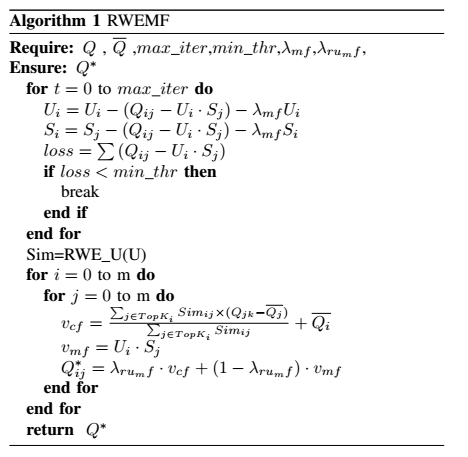
\includegraphics[width=0.45\paperwidth]{alg1.png}
    \end{figure}
 
% ====================================================
\par The time complexity of RWEMF is inherited from CF and MF. With the algorithm RWEMF, the time complexity of CF is from O($m \times n \times n$) to O($m \times n \times K$), where the K is the latent dimension of matrix U. When the n is large and the K is small, the time will be saved in large dataset. Besides, the time complexity of MF is O($m \times n \times l$), where l is the influenced by the max\_iter(maximum iteration) and $d \%$(the density of dataset). In summary, the RWEMF algorithm adds no extra time complexity in those web service dataset. Although its time complexity is large than the sum of CF and MF, the running time\cite{wang_collaborative_2015} is still in acceptable scale even on the large web service dataset.

\begin{figure}[H]
    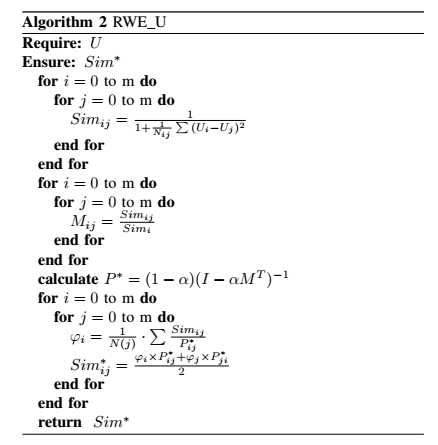
\includegraphics[width=0.45\paperwidth]{alg2.png}
    \end{figure}


%=========================================================================
\section{Experiment and Evaluation}\label{S-EE}
\subsection{Dataset and Description}
The dataset is from WS-DREAM \footnote{github.com/wsdream/wsdream-dataset}. The whole dataset includes two sub-dataset: response time(RT) and throughput(TP). The statistics of dataset are shown in Table \ref{tb1}. The dataset reflects the real-world condition that we have few user-clients to observe the QoS value and there are so many service on the Internet. 
% table=============================================
\begin{table}[H]
\begin{threeparttable}
\caption{Statistics of dataset}
\label{tb1}
\begin{tabular}{c||c|c|c|c|c|c} 
\hline 
QoS & numU & numS & min & max & mean & std \\ 
\hline 
RT(sec) & 339   & 5825  & 0.001 & 19.999 & 0.9086 & 1.9727 \\ 
\hline 
TP(kbps) & 339   & 5825  & 0.004 & 1000  & 47.5617 & 110.7971  \\ 
\hline 
\end{tabular} 
\end{threeparttable}
\end{table}

\par The information about the location of users and services displays in Table \ref{tb2}. The row of ``user\_as'' means there are 339 users in the dataset. And the 339 users are distributing in 136 areas. Every area has at least 1 user and no more than 31 users. And the average number of users on one area about 2.4745 with 2.8338 standard deviation. Notice that the postfix ``\_as" and ``\_ct" means area is as(auto system) and ct(country) respectively. From the statistic information about data, the fact that users or services distribute in different area are extremely unbalance. The dataset of location provides inefficiency information, that is why the location information is difficult to enhance the accuracy of experiments.

% table=============================================
\begin{table}[H]
\begin{threeparttable}
\caption{Statistics of userinfo and serviceinfo}
\label{tb2}
\begin{tabular}{c||c|c||c|c|c|c}
\hline 
infoattr & num & size & min & max & mean & std \\
\hline
user\_as & 339   & 136   & 1     & 31    & 2.4745 & 2.8338 \\
\hline
user\_ct & 339   & 30    & 1     & 161   & 10.9355 & 28.3673 \\
\hline
service\_as & 5825  & 992   & 1     & 1212  & 5.8661 & 40.6092 \\
\hline
service\_ct & 5825  & 73    & 1     & 2395  & 78.7162 & 285.9846 \\
\hline
\end{tabular} 
\end{threeparttable}
\end{table}

\subsection{Evaluation Metric and Parameter}
The MAE(Mean Absolute Error) and NMAE(Normalized Mean Absolute Error) are the common measurable metrics. MAE is defined as 
\begin{equation}
MAE=\frac{1}{N}\sum_{i,j}{|q_{ij}-q^{\hat{}}_{ij}|}
\end{equation}
The NMAE is computed as the MAE normalized by the mean of all values, which is defined as 
\begin{equation}
NMAE=\frac{MAE}{\frac{1}{N}\sum_{i,j}{|q_{ij}}|}
\end{equation}
The MAE reflects the absolute error of the predictions. The NMAE reflects the relative error of the predictions. We can compare the ability of predictions from different dataset by NMAE relatively.

\subsection{Result Accuracy and Comparison}
\par There are several classical recommendation algorithms in the experiments as the comparisons. The result of response time and throughput
 are displayed in Table \ref{tb_rt} and Table \ref{tb_tp} respectively.
\par The comparisons including
\begin{itemize}
\item UPCC is the user-based collaborative filtering algorithm that calculates the similarity between users with Pearson correlation coefficient. In this case of small number of users, the algorithm is fast with short running time. 
\item IPCC is the item-based collaborative filtering algorithm that calculates the similarity between users with Pearson correlation coefficient. In this case of large number of services, the algorithm is slow with long running time. 
\item UIPCC is the hybrid method linearly combines the results of UPCC and IPCC, but the accuracy is more precise than that two. With the running time of total two algorithm, the algorithm is also slow.
\item PMF is matrix factorization\cite{r_salakhutdinov__a_mnih_probability_2007} algorithm with the model of probability. In this case, the process is fast to be convergent to stable state. So the maximum iteration and convergent threshold are significant to keep the running time within acceptable range.
\item RWE is user-based random walk model enhanced by matrix factorization. The reduced-dimension matrix U with k dimensions latent elements, the algorithm is more fast and achieves more accuracy.
\item XEMF is matrix factorization based algorithm. The parameters of XEMF is set to fit the sparse dataset specially. The user latent matrix is also used for RWE and RWEMF.
\item RWEMF is our approach which is more efficient in the experiment. In the base of RWE, the approach successfully combined the prediction from matrix factorization. And its running time is close to matrix factorization.
\end{itemize}

\begin{table}[H]
  \centering
  \caption{The MAE and NMAE of response time prediction}
  \label{tb_rt}
    \begin{tabular}{r||l|rrrr}
\hline
model & DS   & 5\%  & 10\% & 15\% & 20\% \\
\hline
UPCC & MAE  & 0.6159 & 0.5371 & 0.4966 & 0.4737 \\
         & NMAE & 0.6794 & 0.5917 & 0.5471 & 0.5219 \\
\hline
IPCC & MAE  & 0.6805 & 0.6572 & 0.5670 & 0.4955 \\
         & NMAE & 0.7507 & 0.7240 & 0.6246 & 0.5459 \\
\hline
UIPCC & MAE  & 0.6045 & 0.5336 & 0.4879 & 0.4601 \\
         & NMAE & 0.6668 & 0.5879 & 0.5374 & 0.5068 \\
\hline
PMF & MAE  & 0.5704 & 0.4894 & 0.4584 & 0.4390 \\
         & NMAE & 0.6292 & 0.5391 & 0.5050 & 0.4837 \\
\hline
RWE & MAE  & 0.5255 & 0.4735 & 0.4462 & 0.4291 \\
         & NMAE & 0.5797 & 0.5216 & 0.4916 & 0.4727 \\
\hline
XEMF & MAE  & 0.5518 & 0.4891 & 0.4756 & 0.4877 \\
         & NMAE & 0.6087 & 0.5388 & 0.5239 & 0.5373 \\
\hline
RWEMF & MAE  & 0.5068 & 0.4560 & 0.4344 & 0.4251 \\
         & NMAE & 0.5591 & 0.5023 & 0.4786 & 0.4683 \\
\hline
    \end{tabular}
\end{table}


\begin{table}[H]
  \centering
  \caption{The MAE and NMAE of throughput prediction}
  \label{tb_tp}
    \begin{tabular}{r||l|rrrr}
\hline
model & DS & 5\% & 10\% & 15\% & 20\% \\
\hline
UPCC & MAE & 26.8039 & 22.2826 & 20.0274 & 18.689 \\
   & NMAE & 0.5643 & 0.4688 & 0.4212 & 0.3931 \\
\hline
IPCC & MAE & 29.5539 & 29.4531 & 30.1322 & 27.5450 \\
   & NMAE & 0.6222 & 0.6196 & 0.6338 & 0.5794 \\
\hline
UIPCC & MAE & 26.0401 & 21.9952 & 20.0911 & 18.6256 \\
   & NMAE & 0.5483 & 0.4627 & 0.4226 & 0.3918 \\
\hline
PMF & MAE & 22.5499 & 17.9761 & 16.5358 & 15.0594 \\
   & NMAE & 0.4748 & 0.3782 & 0.3478 & 0.3168 \\
\hline
RWE & MAE & 19.4043 & 15.6509 & 14.3058 & 13.5797 \\
   & NMAE & 0.4085 & 0.3293 & 0.3009 & 0.2857 \\
\hline
XEMF & MAE & 21.0512 & 17.2567 & 15.9693 & 15.5798 \\
   & NMAE & 0.4432 & 0.3630 & 0.3359 & 0.3277 \\
\hline
RWEMF & MAE & 18.5121 & 15.1752 & 13.9855 & 13.3388 \\
   & NMAE & 0.3898 & 0.3193 & 0.2942 & 0.2806 \\
\hline
    \end{tabular}
\end{table}

\par Form the experimental results are shown in Table \ref{tb_rt} \ref{tb_tp}, we have some observations. 

\begin{itemize}
\item The matrix factorization based algorithm PMF achieves more accuracy than the user-based or item-based without enhancements algorithms(UPCC,IPCC,UIPCC). 
\item The algorithm (HL-RWE) enhanced by random-walk model achieves more accuracy than the similarity based collaborative filtering algorithms(UPCC,IPCC,UIPCC). So the precision similarity calculation and the appropriate and ranking neighbors selected are the efficient approaches to improve the accuracy.
\item The RWEMF algorithm is more efficient than other algorithms and achieves the best accuracy. The sparse density of 5\% is more appropriate for the algorithm to have better performance than that the dense density is 20\%.
\item In the different sub-dataset, the algorithms achieve different performance. The response-time dataset with value range (0.001-19.999) and standard deviation 1.9727 is with fluctuation about 9.86\%. The throughput dataset with value range (0.004-1000) and standard deviation 110.797 is with fluctuation about 11.08\%. The RWEMF achieves $\frac{0.6794-0.5591}{0.6794}=0.1771$ in rt dataset and $\frac{0.5643-0.3898}{0.5643}=0.3092$ in tp dataset. So the sparse density and the fluctuation in the dataset is the important elements to the accuracy of RWEMF.
\end{itemize}

\subsection{Analysis and Deduction}
\par The significant parameters in RWEMF are top K, the latent dimension of MF, the rate of RW and MF union. 

\par From the Figure \ref{fig_rt},\ref{fig_tp}, the number of nearby neighbors selected obviously effects the accuracy. Although the accuracy tendencies are different in different dataset, the appropriate number of nearby neighbors selected decided the best accuracy in different sparse density. When topK=3, the RWEMF achieves the best accuracy in both response-time and throughput dataset. 

\begin{figure}[H]  
\centering  
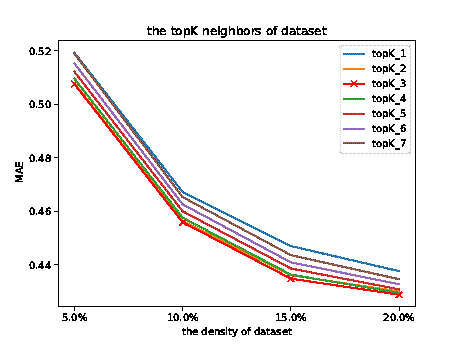
\includegraphics[width=0.45\paperwidth]{topk_rt.png}  
\caption{the MAE of different topK of RWEMF on the response-time dataset }  
\label{fig_rt}  
\end{figure} 

\begin{figure}[H] 
\centering  
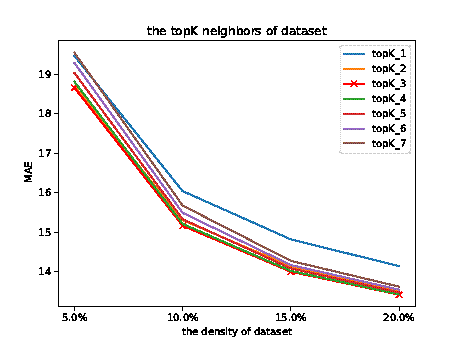
\includegraphics[width=0.45\paperwidth]{topk_tp.png}  
\caption{the MAE of different topK of RWEMF on the throughput dataset }
\label{fig_tp}  
\end{figure} 

\par From the Figure \ref{fig_timae_rt},\ref{fig_timae_tp}, the y-axis on the left shows the running time of the algorithm and the y-axis on the right shows the MAE accuracy of the algorithm. The x-axis represents the latent dimensions in RWEMF. It is clear that different sampling density and the latent dimensions affects the running time. With the two parameters increasing, the running time of the algorithm also increases gradually. At the same time, the MAE accuracy of the algorithm is changing under different latent dimensions. The efficient running of the algorithm requires selecting the appropriate latent dimensions to achieve a balance between computing time and accuracy of prediction. For example, when ldmf = 15, the algorithm runs faster relatively and has higher prediction accuracy.

\begin{figure}[H] 
\centering  
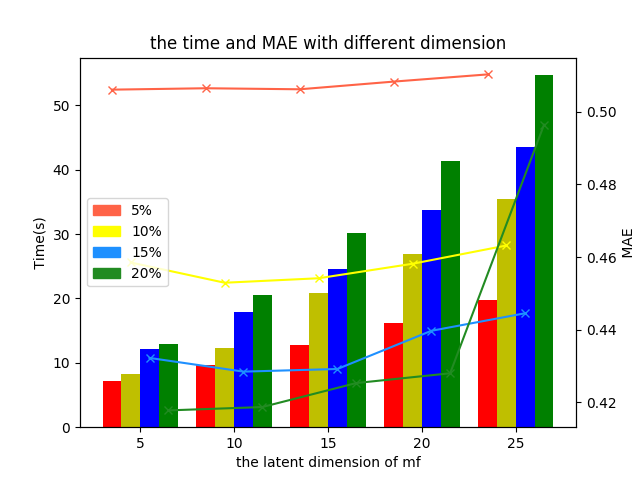
\includegraphics[width=0.45\paperwidth]{timae_rt.png}  
\caption{the running time and MAE of different dimension on the response-time dataset }  
\label{fig_timae_rt}  
\end{figure} 

\begin{figure}[H] 
\centering  
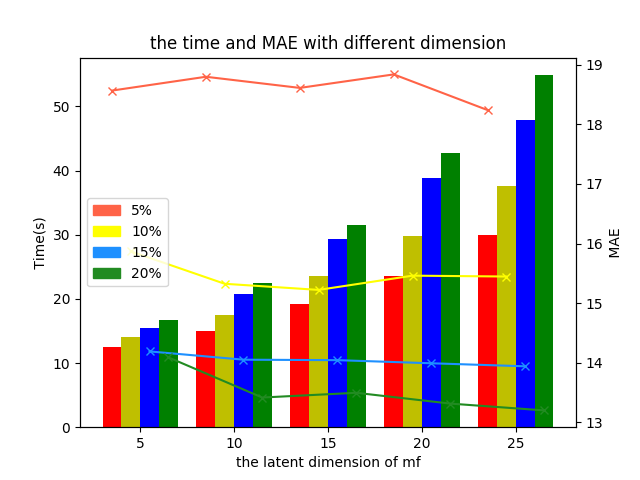
\includegraphics[width=0.45\paperwidth]{timae_tp.png}  
\caption{the running time and MAE of different dimension on the throughput dataset }
\label{fig_timae_tp}  
\end{figure} 

\par From the Figure \ref{fig_rumf_rt},\ref{fig_rumf_tp}, the $\lambda_{rumf}$ parameter is the rate united the MF. In the experiments, we choose the 5\% and 20\% density. And every rate of density has three type lines (including the RWE, XEMF and RWEMF line). It is clearly to see, the MAE of XEMF is the largest in three, the MAE of RWE is smaller than MF's. With the 0.7 of $\lambda_{rumf}$, the RWEMF reaches the best accuracy of MAE. The phenomenon is the same in the throughput dataset. But the response-time dataset with small value is more sensitive to the rate, and it reaches the best accuracy in short range. 


\begin{figure}[H] 
\centering  
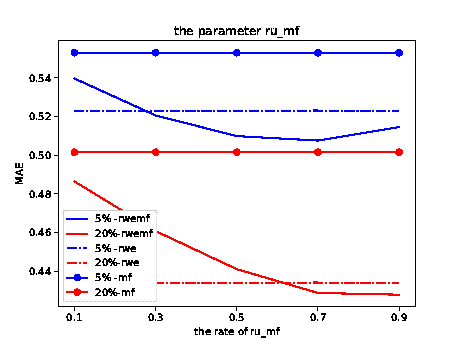
\includegraphics[width=0.45\paperwidth]{rumf_rt.png}  
\caption{the MAE of different rate union MF on the response-time dataset }  
\label{fig_rumf_rt}  
\end{figure} 

\begin{figure}[H] 
\centering  
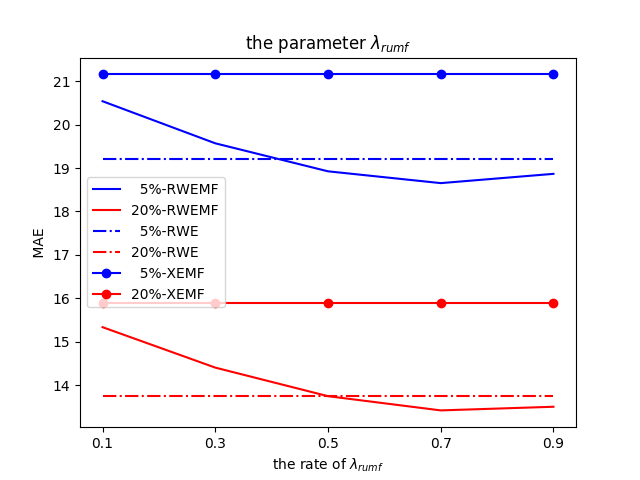
\includegraphics[width=0.45\paperwidth]{rumf_tp.png}  
\caption{the MAE of different rate union MF  on the throughput dataset }
\label{fig_rumf_tp}  
\end{figure} 

\par Every point in Figure \ref{fig_ae_rt},\ref{fig_ae_tp} means the prediction of three algorithm(RWEMF,RWE,MF) minus the real QoS value of dataset, and the points in view are sampled randomly that on behalf of the whole predictions. It is easy to see the AE(Absolute Error) reflects the accuracy of points. And the points of RWEMF are locating in the middle between RWE and MF. Sometimes the RWE gets the more accuracy, but it also undergoes with the big variance. And the MF can not get the more accuracy, but it also runs steadily with the small variance. And the predictions of algorithms are sensitive to value of dataset. The AE in throughput dataset fluctuated in large range compared to response-time dataset.

\begin{figure}[H] 
\centering  
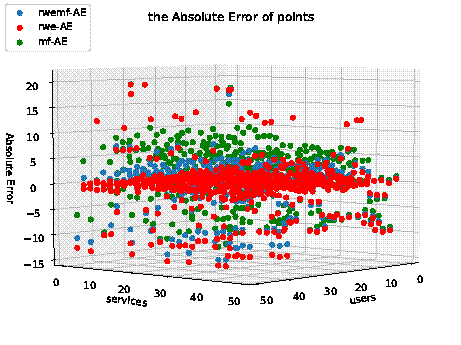
\includegraphics[width=0.45\paperwidth]{ae_rt.png}  
\caption{the Absolute Error on the response-time dataset }  
\label{fig_ae_rt}  
\end{figure} 

\begin{figure}[H] 
\centering  
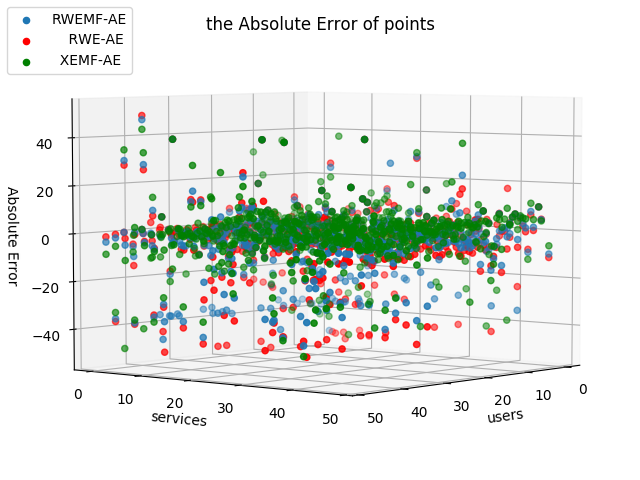
\includegraphics[width=0.45\paperwidth]{ae_tp.png}  
\caption{the Absolute Error on the throughput dataset }  
\label{fig_ae_tp}  
\end{figure} 

%=========================================================================
\section{Conclusion}\label{S-CN}
\par We propose RWEMF a hybrid approach to achieve best accuracy of prediction in QoS real-world web service dataset. Firstly, We recognize sparse dataset through statistics information. Clearly, the similar calculation and the nearby neighborhood selection are significant. And the combination of random-walk based collaborative filtering and matrix factorization algorithm are described in this paper. The experiments of RWEMF prove that our algorithm is most efficient, and the best parameters chosen are important to get the best accuracy in this dataset.
\par In the future, the RWEMF with the best accuracy in this dataset can be extended by more efficient model. The short running time and exquisite mind can help the algorithm being used in real-world web service recommendation easily. The parameters for the hybrid model need more exploration and more study to keep the algorithm more efficient. Although the adherent information of users and service improve the accuracy finitely, there are still more latent information\cite{liu_incorporating_2015}  value should be mined in the dataset. The MAE on 5\% on response-time dataset is 0.5068 now, and the MAE value is relative, however it is good metrics to measure the ability of algorithm in sparse dataset. Further, the MAE would be lower that 0.5000 by the new hybrid model.

%=========================================================================
\section*{Acknowledgment}
The authors would like to thank...
 % \cite{liu_location-aware_2016} 
 % \cite{yin_network_2017} 
 % \cite{yu_personalized_2014} 
 % \cite{ma_predicting_2015} 
 % \cite{zheng_wsrec:_2009} 
 % \cite{zheng_qos-aware_2011} 
 % \cite{park_comparative_2017} 
 % \cite{rodriguez-mier_hybrid_2017} 
 % \cite{choi_statistical_2015} 
 % \cite{agarwal_stochastic_2014} 
 % \cite{zhou_qos-aware_2015} 
 % \cite{xia_domain-aware_2014} 
 % \cite{wang_collaborative_2015} 
 % \cite{liu_incorporating_2015} 
 % \cite{tang_location-aware_2012} 
 % \cite{lo_efficient_2014} 
 % \cite{chen_user_2016} 
 % \cite{r_salakhutdinov__a_mnih_probability_2007} 
 % \cite{hadad_tqos:_2010} 
 % \cite{mohammed_markov_2016} 
 % \cite{tran_low-rank_2016} 
 % \cite{ongie_fast_2017} 
 % \cite{koren_matrix_2009}

\bibliographystyle{IEEEtran}
\bibliography{IEEEabrv,rwemfbib}

% \begin{thebibliography}{1}
% \input{rwemfbib.bib}
% % \bibitem{IEEEhowto:kopka}
% % H.~Kopka and P.~W. Daly, \emph{A Guide to \LaTeX}, 3rd~ed.\hskip 1em plus
% %   0.5em minus 0.4em\relax Harlow, England: Addison-Wesley, 1999.

% \end{thebibliography}

\end{document}

